\documentclass{article}
\usepackage{microtype}
\usepackage{graphicx}
\usepackage{booktabs}
\usepackage{hyperref}
\usepackage{amsmath}
\usepackage{amssymb}
\usepackage{algorithm}
\usepackage{algorithmic}
\usepackage{xcolor}
\usepackage[margin=1in]{geometry}

\title{Advancing Knotted Protein Design with ESM3:\\Guided Generation and Topological Insights}

\author{
   Eva Marsalkova \\
   CEITEC \& National Centre for Biomolecular Research\\
   Masaryk University, Brno, Czech Republic 
  \and
  Petr Simecek\thanks{Corresponding author: \texttt{simecek@mail.muni.cz}} \\
  Central European Institute of Technology (CEITEC)\\
  Masaryk University, Brno, Czech Republic
}

\date{}

\begin{document}
\maketitle

\begin{abstract}
Multimodal protein language models have transformed protein design, yet their capacity to capture complex topological features remains poorly understood. We use knotted proteins, rare structures in which the backbone forms a nontrivial topological knot, as a test case to probe this capacity using ESM3, a generative protein language model. ESM3's guided generation produces knotted proteins with an 89\% success rate (95\% CI: 81--94\%), compared to $\sim$0.5\% for unguided diffusion-based approaches. Knot topology is remarkably robust to sequence perturbation: on average 84\% of the protein sequence must be altered before the knot breaks, and the loss follows a sharp threshold rather than gradual degradation. Strikingly, structural drift accumulates well before topological disruption, suggesting that topology is more robust than specific three-dimensional arrangement. Generated proteins show no close sequence similarity to known knotted proteins, arguing against simple memorization. These findings have implications for protein engineering and, more speculatively, for discussions of biosecurity in the era of generative biological AI.
\end{abstract}

%=====================================================================
\section{Introduction}
%=====================================================================

Recent years have seen remarkable progress in AI-driven protein design. Structure prediction models such as AlphaFold2 \cite{abramson2024accurate} and ESMFold \cite{lin2023evolutionary} predict three-dimensional structures with near-experimental accuracy, while generative tools including RFdiffusion \cite{watson2023novo}, ProteinMPNN \cite{dauparas2022robust}, and EvoDiff \cite{alamdari2023protein} enable the de novo design of proteins with desired structural properties. Multimodal foundation models like ESM3 \cite{hayes2025simulating} integrate sequence, structure, and function information in a single framework, further expanding the design space.

Despite these advances, an important question remains: to what extent do these models capture \emph{topological} features of protein structure? Topology describes aspects of protein architecture that are more fundamental than specific atomic coordinates, namely properties preserved under continuous deformation. A particularly fascinating topological feature in proteins is the knot: a configuration in which the polypeptide backbone forms a nontrivial topological knot that cannot be untied without breaking covalent bonds \cite{taylor2000protein,virnau2006intricate}.

\begin{figure}[t]
\centering
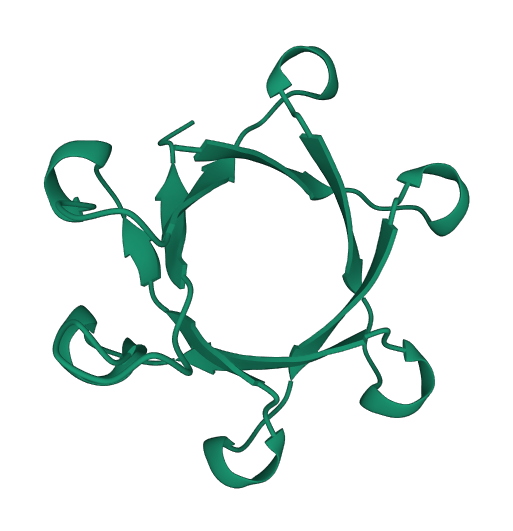
\includegraphics[width=0.4\textwidth]{figures/fig_example_knotted.png}
\caption{Example of a knotted protein (A0A165M1R5, \textit{Acidovorax} sp.), featuring a $7_1$ knot. Imagine pulling on both ends of the polypeptide chain: if the protein is knotted, it will not come apart.}
\label{fig:example}
\end{figure}

Knotted proteins are rare, occurring in less than 1\% of known structures, yet they exhibit enhanced kinetic stability \cite{lua2012pyknot,sulkowska2012stabilizing}, resistance to proteolytic degradation \cite{soler2013effects}, and unique functional properties \cite{king2007identification,brems2022alphafold}. Their strong evolutionary conservation suggests functional importance \cite{sulkowska2012conservation,begun2024effect}. Databases such as KnotProt \cite{dabrowski2019knotprot} and AlphaKnot \cite{alphaknot} catalogue the growing repertoire of known knotted topologies, while computational tools like Topoly \cite{topoly} enable their detection using polynomial invariants. Recent work by Klimentov\'{a} et al.\ \cite{klimentova2024unveiling} demonstrated that diffusion-based protein design can generate artificial knotted proteins, though with a success rate of approximately 0.5\%.

The ability of generative models to reconstruct complex protein structures from partial information also raises questions for biosecurity. It is common practice to redact or delete portions of sensitive protein sequences before publication to reduce dual-use risks \cite{lewis2020biosecurity_attribution}. Knotted proteins offer an ideal model system to study the effectiveness of such redaction: they are structurally complex, require precise spatial arrangements, have clear detection criteria, yet are not themselves harmful, allowing rigorous experimentation without biosafety concerns.

In this work, we leverage ESM3 to systematically investigate how protein language models interact with topological complexity. While we use only the smallest open-source variant (ESM3-SM, 1.4B parameters), we believe the results illustrate general principles about the relationship between learned representations and protein topology.

%=====================================================================
\section{Methods}
%=====================================================================

\subsection{Dataset}

We use the publicly available \texttt{EvaKlimentova/Diffusion-all\_knots} dataset \cite{klimentova2024unveiling}, containing 15,000 proteins from three sources (Real, RFdiffusion-generated, EvoDiff-generated), each with 1,000 knotted and 4,000 unknotted proteins. We focus on the 5,000 real proteins (1,000 knotted, 4,000 unknotted). The knotted proteins have a mean sequence length of 399 residues (median 340, std 196, range 80--1000); the unknotted proteins have comparable statistics (mean 405, median 339, std 204). All knotted proteins were verified against the AlphaKnot 2.0 database \cite{alphaknot}, confirming knot types and core positions; the predominant type is the trefoil ($3_1$).

\subsection{ESM3 Model and Guided Generation}

We employ ESM3-SM (1.4B parameters) \cite{hayes2025simulating} in half precision (fp16) on NVIDIA A10G GPUs via Modal serverless compute. ESM3 is a generative masked language model that reasons jointly across sequence, structure, and function tracks, enabling iterative unmasking of partially specified proteins. Given a partially masked protein, the model predicts probability distributions over tokens at masked positions; iterating this process progressively fills in the complete protein.

For guided generation, we use derivative-free guided decoding \cite{dfg_diffusion} as implemented in the ESM3 SDK. At each decoding step, multiple candidate unmaskings are sampled and scored by a user-defined objective; the highest-scoring candidate is kept, and the process repeats. We define a knot scoring function $s(x)$ using the Topoly Python package \cite{topoly} with Alexander polynomials. Topoly uses stochastic closure (projecting the open protein chain along random directions to form closed curves), yielding a probability distribution over topological types. With $N_{\text{proj}}=30$ random projections, the score is:
\begin{equation}
s(x) = 1 - \frac{P(\text{topology} = 0_1)}{\sum_k P(\text{topology} = k)}
\end{equation}
where $0_1$ denotes the trivial (unknotted) topology, and $P(\text{topology}=k)$ is the fraction of stochastic closures yielding topology $k$. For de novo generation, we start from a fully masked sequence of length 256 and apply 8 decoding steps with 10 candidate samples per step, selecting the candidate with the highest knot score at each step.

\subsection{Continuous Knot Score and Masking Strategies}

We propose a continuous knot score based on randomized masking (Algorithm~\ref{alg:knot_score}). For each protein, we randomly replace $X$\% of residues with mask tokens, use ESM3 to regenerate the masked positions (8 generation steps, temperature 1.0), predict the structure of the resulting sequence (8 structure generation steps), and evaluate topology via Topoly. Averaging over $N=8$ independent trials yields a score in $[0, 1]$. We systematically vary $X$ from 10\% to 90\%.

\begin{algorithm}[tb]
   \caption{Randomized Knot Score Calculation}
   \label{alg:knot_score}
\begin{algorithmic}
   \STATE {\bfseries Input:} protein sequence $s$, masking percentage $X$, trials $N$
   \STATE {\bfseries Output:} knot\_score $\in [0, 1]$
   \STATE $\text{knotted\_sum} \leftarrow 0$
   \FOR{$i=1$ {\bfseries to} $N$}
   \STATE Randomly replace $X$\% of residues in $s$ with mask tokens
   \STATE Regenerate masked positions using ESM3 (8 steps, temperature 1.0)
   \STATE Predict structure using ESM3 (8 steps)
   \STATE Compute topology via Topoly ($N_{\text{proj}}=30$ stochastic closures)
   \STATE $\text{knotted\_sum} \mathrel{+}= \text{fraction of closures with nontrivial topology}$
   \ENDFOR
   \STATE {\bfseries Return} $\text{knotted\_sum} / N$
\end{algorithmic}
\end{algorithm}

We compare three masking strategies: \textbf{random masking} (uniformly sampled positions), \textbf{contiguous masking} (a single block), and \textbf{targeted masking} of the knot core versus flanking regions, using ground-truth core positions from AlphaKnot 2.0.

\subsection{Structural Drift and Embedding Analysis}

We measure backbone RMSD between the ESM3-predicted structure of the original sequence and the ESM3-predicted structure after masking and regeneration, using the Aligner utility from the ESM3 package (C$\alpha$ atom superposition). The RMSD analysis uses a smaller sample ($n=80$) than the masking analysis ($n=250$) because each RMSD measurement requires generating and aligning two full structures, making it computationally more expensive. We also compute pairwise sequence identity as the fraction of matching residues at aligned positions, normalized by the length of the longer sequence.

For embedding analysis, we extract mean-pooled ESM3 embeddings (dimension 1,536) from protein sequences and train a multilayer perceptron with two hidden layers (1,024 and 256 neurons, ReLU activation) for binary classification (knotted vs.\ unknotted), using an 80/20 stratified train/validation split (4,000 train, 1,000 validation) with early stopping on validation loss (scikit-learn MLPClassifier).

%=====================================================================
\section{Results}
%=====================================================================

\subsection{Guided Generation of Knotted Proteins}

ESM3's guided generation achieved an 89\% success rate (89/100; 95\% CI: 81--94\%) in producing knotted proteins from fully masked sequences, compared to the $\sim$0.5\% success rate reported for unguided diffusion-based approaches \cite{klimentova2024unveiling}. We note that this comparison is between guided and unguided generation and should be interpreted accordingly: the improvement reflects the effectiveness of guided decoding with a topology-aware scoring function, not a direct comparison of model architectures.

Among the 70 proteins with resolved knot types (the remaining 19 exceeded the Alexander polynomial's default crossing limit of 15 and could not be classified; see Limitations), trefoil knots ($3_1$) were most common (33 occurrences), followed by figure-eight knots ($4_1$, 10) and torus knots ($5_2$, 10). More complex types including $8_{19}$, $9_{44}$, and $9_{45}$ were also generated (Figure~\ref{fig:knot_types}).

\begin{figure}[t]
\centering
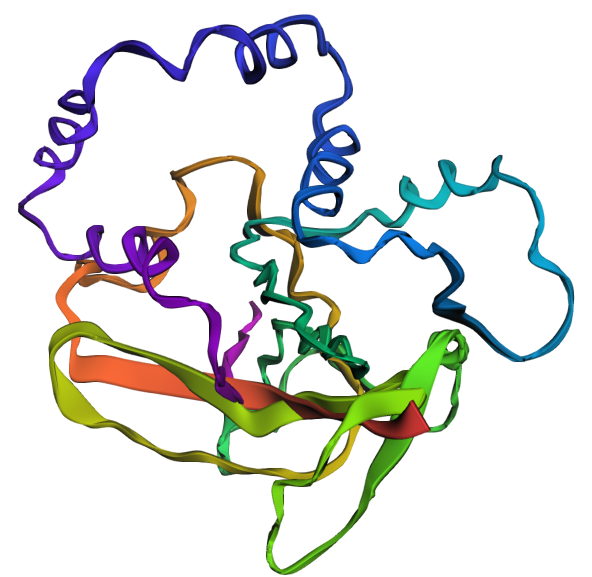
\includegraphics[width=0.42\textwidth]{figures/fig_generated_example.png}\hfill
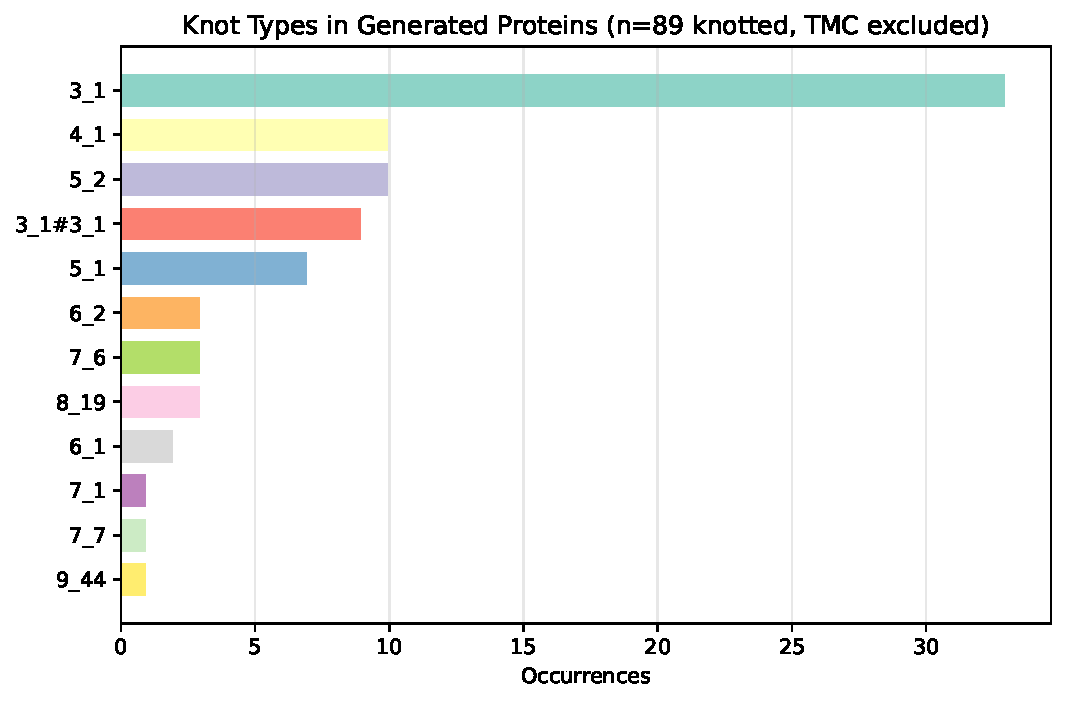
\includegraphics[width=0.55\textwidth]{figures/fig_knot_types.pdf}
\caption{Left: example de novo generated knotted protein. Right: distribution of resolved knot types in successfully generated proteins. The trefoil ($3_1$), the simplest and most common knot in natural proteins, dominates, but complex topologies with up to 9 crossings are also produced.}
\label{fig:knot_types}
\end{figure}

We further tested knot-type-specific generation by modifying the scoring function to preferentially reward a particular topology. Targeting the trefoil was highly effective (9/10 hit the target), consistent with $3_1$ being the simplest and most common knot type. When the model generates a knot but misses the target, it naturally defaults to the most probable topology. More complex targets ($4_1$, $5_1$, $5_2$) were achieved in 20--30\% of attempts, with generation biased toward trefoils in the remaining cases (Supplementary Figure~S9). The success rate also depends on target protein length: at 100 residues only 20\% of attempts produced knots, rising to 90\% at 200 residues and 100\% at 350 or more (Supplementary Figure~S1), consistent with the observation that natural knotted proteins are typically 200--400 residues long.

A simple MLP classifier trained on mean-pooled ESM3 embeddings achieves 97.1\% accuracy in distinguishing knotted from unknotted proteins ($n_\text{val}=1000$; Supplementary Figure~S6), suggesting that ESM3's learned representations encode information relevant to topology even without explicit topological supervision.

\subsection{Knot Robustness and Sharp Threshold Behavior}

Our masking stability analysis ($n=250$ proteins, 10 masking levels, 8 trials each) reveals that knot topology is remarkably stable under sequence perturbation (Figure~\ref{fig:masking_curve}). At 50\% masking, 94\% of knotted proteins retain their topology. At 70\% masking, where only 30\% of the original sequence remains, 85\% are still knotted. The mean breaking point is 84\% ($\pm$ 1.2\% SE).

\begin{figure}[t]
\centering
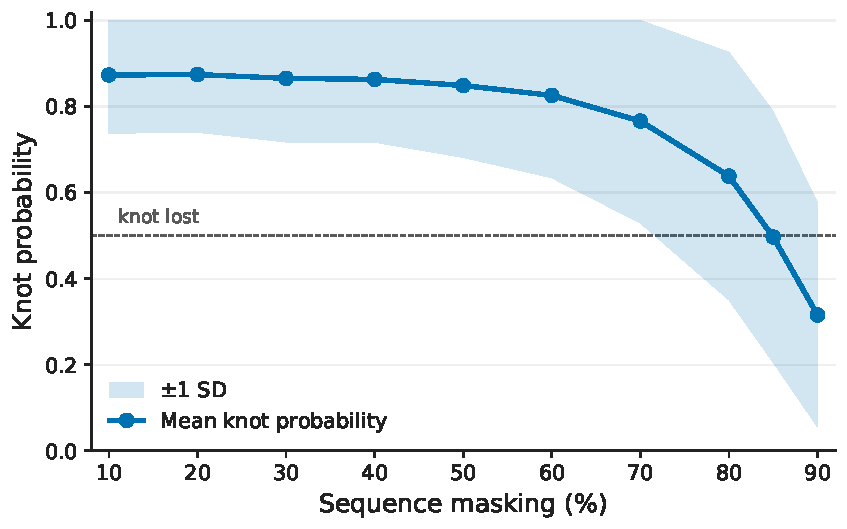
\includegraphics[width=0.9\textwidth]{figures/fig_masking_curve.pdf}
\caption{Knot probability as a function of masking percentage ($n=250$). Shading shows $\pm1$ standard deviation. The knot persists until approximately 80--90\% of the sequence is masked, then drops sharply.}
\label{fig:masking_curve}
\end{figure}

The loss of topology appears abrupt rather than gradual: 68\% of proteins exhibit a single-step drop in knot probability exceeding 0.3 between consecutive masking levels (Supplementary Figure~S2). While the 10-percentage-point spacing of our masking grid limits our ability to distinguish a true discontinuity from a steep sigmoid, the behavior is consistent with a sharp threshold-like transition, suggesting a critical amount of sequence information is required to specify the topology.

\subsection{Structural Drift Precedes Topological Disruption}

The RMSD analysis ($n=80$; smaller than the masking analysis due to the additional computational cost of structure generation and alignment) reveals a key decoupling between structural conservation and topological persistence (Figure~\ref{fig:rmsd}). At 50\% masking, the median RMSD is already 3.24\,\AA{} and sequence identity has dropped to 73\%, yet the mean knot probability remains 0.85. At 70\% masking, RMSD reaches 4.58\,\AA{} (substantial structural rearrangement), while the knot probability is still 0.76.

\begin{figure}[t]
\centering
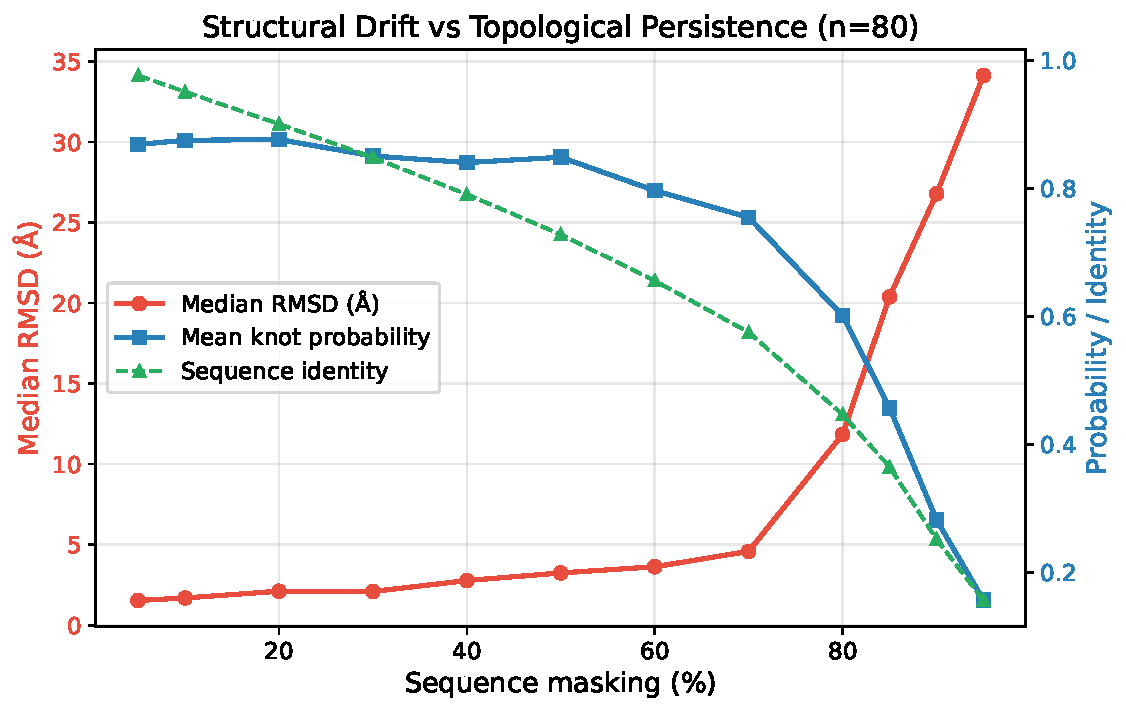
\includegraphics[width=0.9\textwidth]{figures/fig_rmsd_vs_knot.pdf}
\caption{Structural drift (RMSD, red) accumulates steadily with masking, while knot topology (blue) persists until much higher masking levels. Sequence identity (green) declines monotonically. The gap between the curves suggests that topology is more robust than specific 3D arrangement.}
\label{fig:rmsd}
\end{figure}

This decoupling suggests that topology is more robust than specific three-dimensional arrangement. The model generates structures that differ substantially from the original in atomic coordinates yet maintain the same topological class, consistent with the idea that the knot is encoded in a distributed manner across the sequence, with many different conformations capable of realizing the same topology.

\subsection{Evidence Against Simple Memorization}

One might worry that the model simply memorizes and retrieves knotted sequences from its training data rather than capturing nontrivial information about topology. Several lines of evidence argue against this interpretation.

First, de novo generation starts from a fully masked sequence, so there is no input information to trigger retrieval. Second, the generated knotted proteins show no close sequence similarity to known knotted proteins (Figure~\ref{fig:novelty}): the maximum identity between any generated protein and any of the 1,000 known knotted proteins in the dataset is just 14.5\%, with a mean of 10.5\%, indistinguishable from the random baseline of 10.4\% (random unknotted proteins compared to the same knotted set). Not a single generated protein exceeds 20\% identity with any known knotted protein.

\begin{figure}[t]
\centering
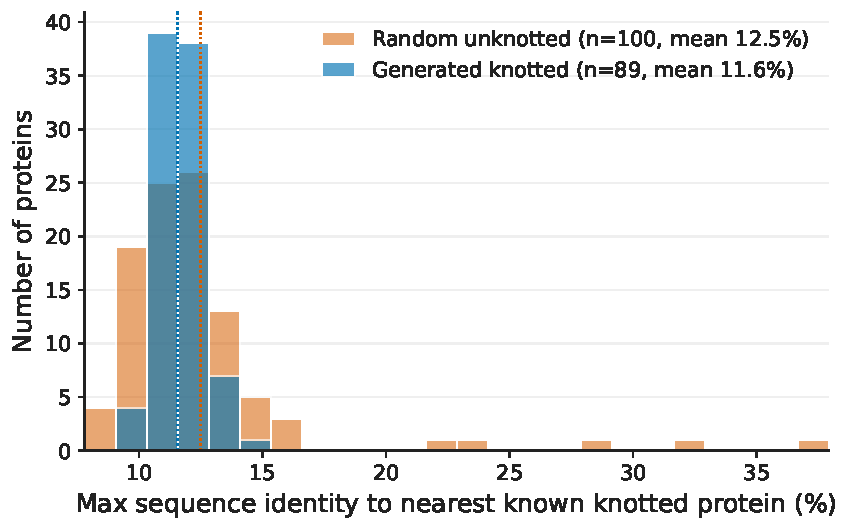
\includegraphics[width=0.9\textwidth]{figures/fig_novelty.pdf}
\caption{Maximum sequence identity of each generated knotted protein to its nearest known knotted protein (blue), compared to random unknotted proteins (red baseline). The distributions overlap completely, indicating that generated proteins are no more similar to known knotted proteins than random sequences are.}
\label{fig:novelty}
\end{figure}

Third, at 50\% masking the regenerated sequences share only 73\% identity with the originals yet maintain 85\% knot probability (Supplementary Figure~S3). We note that low sequence identity does not by itself exclude structural similarity (two proteins can share very different sequences yet similar folds); however, the combination of novel sequence, novel generation context (all-mask input), and the ability to steer generation toward specific knot types via modified scoring functions collectively argues against simple template retrieval.

\subsection{Unknotted-to-Knotted Conversion}

Using iterative guided generation with low-rate masking (3\% per iteration, up to 15 iterations), we converted 17 out of 99 unknotted proteins ($\leq$250 residues) into knotted variants, achieving a 17\% success rate (95\% CI: 10--26\%). This is substantially higher than the $\sim$0.5\% rate achievable without guided generation \cite{klimentova2024unveiling}. Successful conversions showed a bimodal pattern: 8 proteins converted within 3 iterations, while 9 required 7--14 iterations. The remaining 82 proteins showed almost no progress (61 scored exactly 0.0), suggesting that most unknotted proteins are strongly resistant to topological transformation. We did not evaluate the physical plausibility (e.g., pLDDT scores) of the converted structures, which remains an important direction for future work.

\begin{table}[t]
\caption{Summary of key results.}
\label{tab:summary}
\begin{center}
\begin{small}
\begin{tabular}{lrl}
\toprule
Experiment & Result & 95\% CI \\
\midrule
Guided generation success rate & 89\% ($n=100$) & [81, 94\%] \\
Mean breaking point (masking) & 84\% ($n=250$) & $\pm$ 1.2\% SE \\
Knotted at 70\% masking & 85\% of proteins & --- \\
RMSD at 50\% masking & 3.24\,\AA{} median ($n=80$) & --- \\
Max seq.\ identity to known knotted & 14.5\% ($n=89$) & --- \\
Embedding classifier accuracy & 97.1\% ($n_\text{val}=1000$) & --- \\
Unknotted-to-knotted conversion & 17\% ($n=99$) & [10, 26\%] \\
\bottomrule
\end{tabular}
\end{small}
\end{center}
\end{table}

Additional results on targeted core masking, contiguous versus random masking, sliding window vulnerability profiles, embedding-based classification, and UMAP visualization of the embedding space are presented in the Supplementary Materials.

%=====================================================================
\section{Discussion}
%=====================================================================

Our results suggest that multimodal protein language models capture nontrivial information about protein topology, even in their smallest variants. The 89\% success rate in guided knotted protein generation, combined with the diversity of generated topologies, indicates that ESM3 can be effectively steered toward rare and complex structural targets. The ability to generate proteins with knot types containing up to 9 crossings, topologies that are rare or absent in natural proteins, opens possibilities for engineering proteins with novel mechanical and functional properties \cite{strassler2022tied,sulkowska2012stabilizing}.

The sharp threshold behavior in knot stability is perhaps our most striking finding. Rather than a gradual degradation, most proteins show an abrupt loss of topology at a critical masking threshold. One interpretation is that topological information is distributed and partially redundant across the sequence: above a critical information threshold the model can reconstruct the knot; below it, the topology is rapidly lost. The decoupling between RMSD and topology, where structures diverge substantially in 3D space while maintaining the same knot type, further supports the view that topology is a more fundamental feature than specific atomic arrangement, consistent with the mathematical nature of topological invariants.

These findings also have potential implications for biosecurity. Current practices of redacting portions of sensitive protein sequences assume that partial information is insufficient for reconstruction. Our results show that after masking 70\% of a sequence, modern generative models can still recover complex topological features with 85\% reliability. Targeted deletion of the knot core still allows reconstruction 66\% of the time from flanking context alone (Supplementary Table~S1). We emphasize several caveats: our experiments use random and block masking, which differs from real-world targeted redaction of specific functional regions; the threat model is not fully developed; and we do not claim that knotted proteins themselves pose biosecurity risks. Rather, the results suggest that the effectiveness of sequence redaction as a general safeguard deserves further scrutiny in the context of increasingly capable generative models.

\paragraph{Limitations.} Our experiments use ESM3-SM (1.4B parameters), the smallest publicly available variant; larger models (7B, 98B) would likely show stronger capabilities. All topology detection is computational (Alexander polynomials via stochastic closure); we did not perform wet-lab validation of generated proteins, nor did we assess their physical plausibility beyond topology (e.g., energy minimization, pLDDT scores). Approximately 21\% of generated knotted proteins (19/89) had topologies too complex for the Alexander polynomial to resolve within the default crossing limit of 15; using HOMFLY-PT or Jones polynomials could potentially disambiguate these cases. The unknotted-to-knotted conversion rate (17\%) is modest, and the bimodal success pattern suggests fundamental limitations of iterative guided generation for topological transformation.

\paragraph{What this study does not show.} We do not demonstrate that ESM3 ``understands'' topology in a mathematical sense. The model may have learned statistical regularities in sequence--structure relationships that happen to correlate with topological features, without representing topology explicitly. We also do not demonstrate biosecurity risks from knotted proteins specifically; they serve as a model system. Extension of these findings to actual dual-use scenarios would require additional analysis with realistic threat models.

\paragraph{Future work.} Key directions include experimental validation of generated knotted proteins, extension to other complex structural features (slipknots, lasso motifs \cite{dabrowski2019knotprot}), systematic study of what sequence features make a protein amenable to topological transformation, and information-theoretic analysis of the minimum sequence information required to specify a given topology. Testing with larger ESM3 variants as they become publicly available would clarify whether the observed capabilities scale with model size.

%=====================================================================
\section{Conclusion}
%=====================================================================

We have investigated the interaction between multimodal protein language models and topological complexity, using knotted proteins as a test case. Our key findings are:

\begin{itemize}
    \item ESM3-guided generation produces knotted proteins with an 89\% success rate and diverse topology, compared to $\sim$0.5\% for unguided approaches.
    \item Knot topology exhibits a sharp threshold-like behavior under sequence perturbation: on average 84\% of the sequence must be altered before the knot breaks.
    \item Structural drift (RMSD) precedes topological disruption, suggesting that topology is more robust than specific 3D arrangement.
    \item Generated knotted proteins show no close sequence similarity to known knotted proteins (mean 10.5\%, indistinguishable from random), arguing against simple memorization.
\end{itemize}

These results are consistent with the view that protein language models capture nontrivial information related to topology. As such models continue to scale, understanding their topological capabilities becomes increasingly important, both for harnessing their potential in protein design and for anticipating challenges in biosafety governance.

%=====================================================================
\section*{Data and Code Availability}
%=====================================================================
All code used in this study is publicly available at \url{https://github.com/ML-Bioinfo-CEITEC/KPDwESM3}. The dataset is available at \url{https://huggingface.co/datasets/EvaKlimentova/Diffusion-all_knots}.

%=====================================================================
\section*{Acknowledgments}
%=====================================================================
The project was supported by the OPUS LAP program of the Czech Science Foundation, project no.\ 23-04260L (``Biological code of knots -- identification of knotted patterns in biomolecules via AI approach''). Computational resources were provided by Modal serverless GPU compute.

\bibliographystyle{plain}
\bibliography{references}

%=====================================================================
\appendix
\section*{Supplementary Materials}
%=====================================================================

\renewcommand{\thefigure}{S\arabic{figure}}
\renewcommand{\thetable}{S\arabic{table}}
\setcounter{figure}{0}
\setcounter{table}{0}

\begin{figure}[h]
\centering
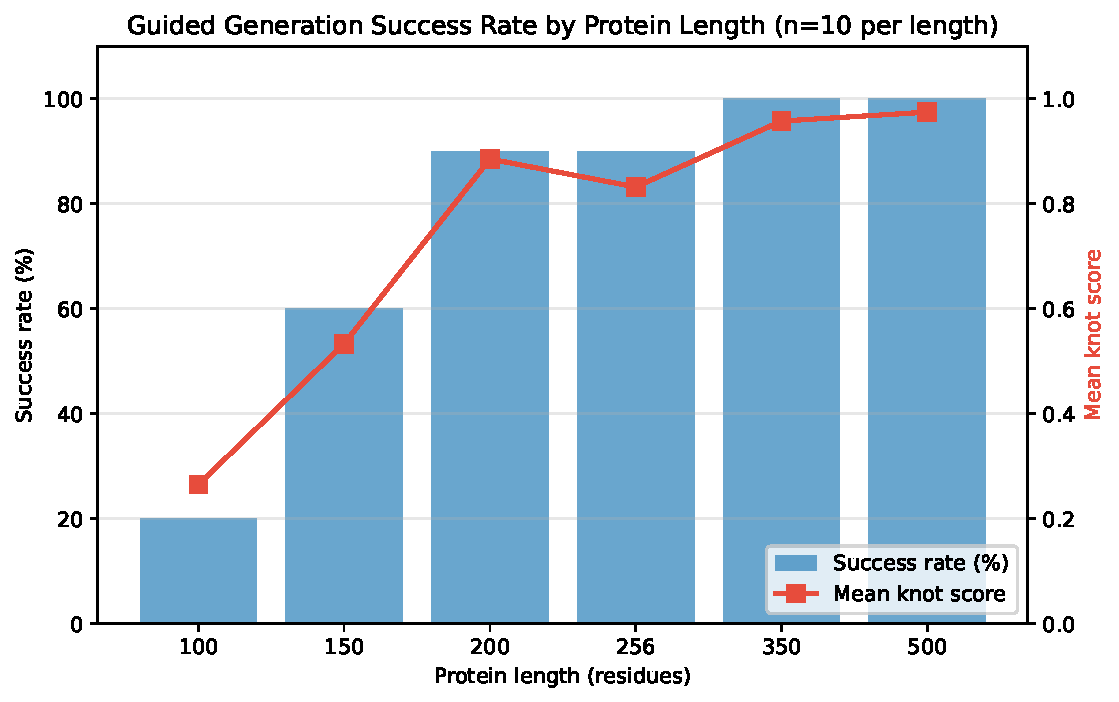
\includegraphics[width=0.85\textwidth]{figures/fig_length_gen.pdf}
\caption{Guided generation success rate by target protein length ($n=10$ per length).}
\label{fig:length_gen}
\end{figure}

\begin{figure}[h]
\centering
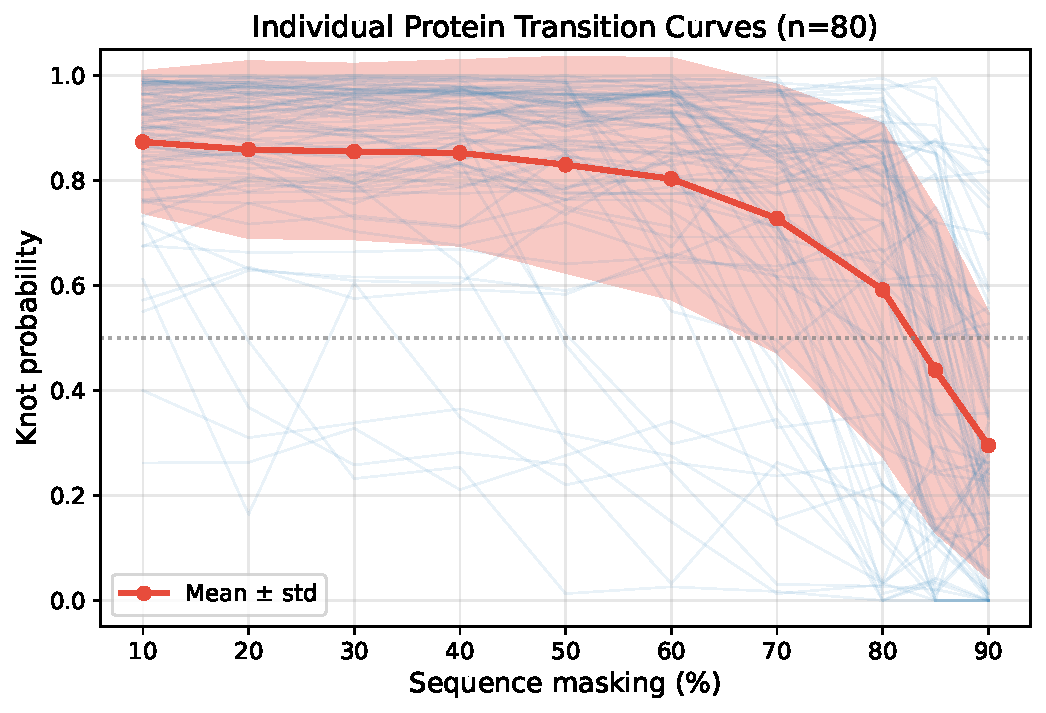
\includegraphics[width=0.9\textwidth]{figures/fig_transition_curves.pdf}
\caption{Individual protein transition curves (blue, low opacity) overlaid with the population mean (red).}
\label{fig:transition}
\end{figure}

\begin{figure}[h]
\centering
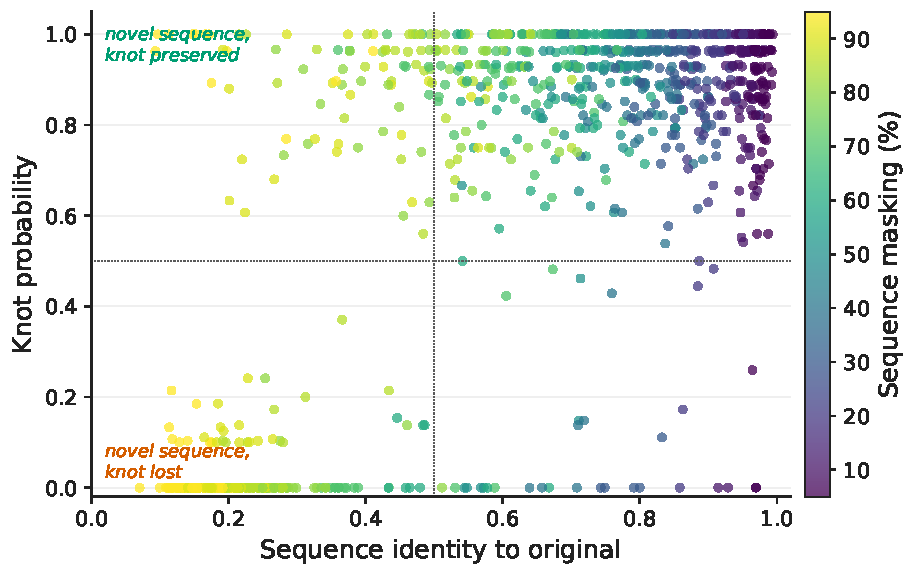
\includegraphics[width=0.9\textwidth]{figures/fig_identity_vs_knot.pdf}
\caption{Per-protein sequence identity versus knot probability at different masking levels.}
\label{fig:identity}
\end{figure}

\begin{figure}[h]
\centering
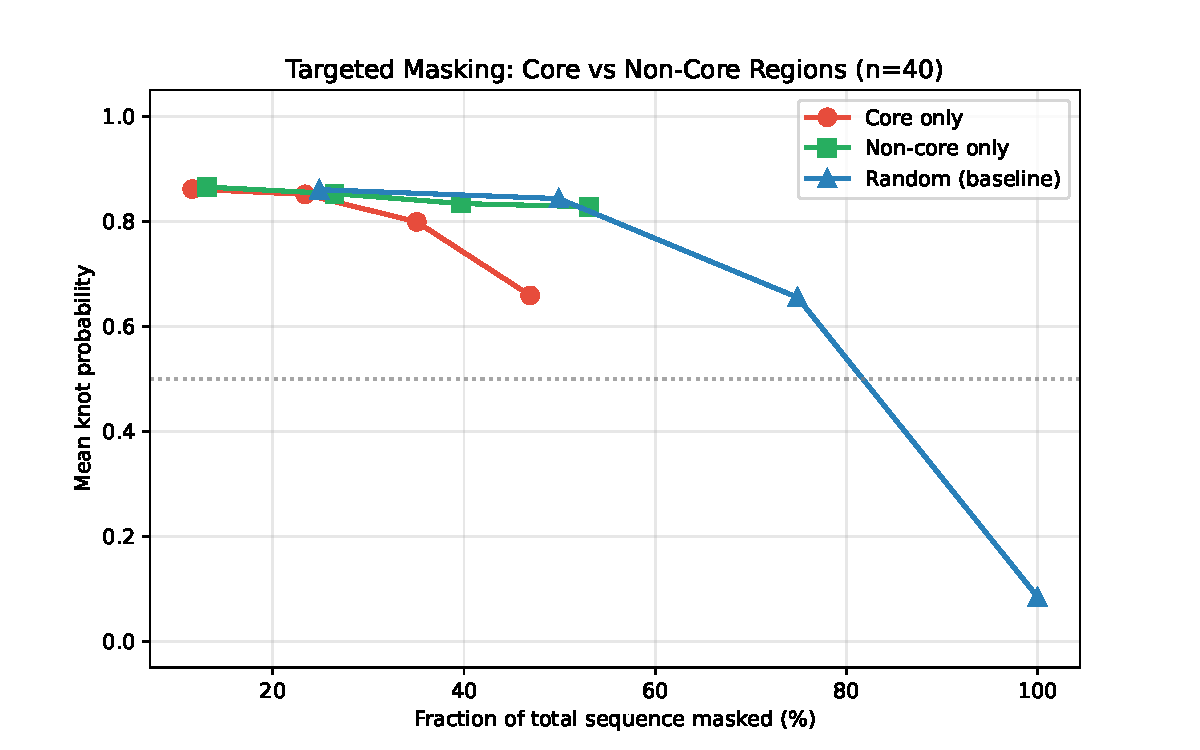
\includegraphics[width=0.9\textwidth]{figures/fig_targeted_masking.pdf}
\caption{Targeted masking of knot core versus non-core regions versus random masking.}
\label{fig:targeted}
\end{figure}

\begin{table}[h]
\caption{Targeted masking: core vs.\ non-core regions ($n=40$).}
\label{tab:targeted}
\begin{center}
\begin{small}
\begin{tabular}{lcc}
\toprule
Region masked & \% of total seq & Mean knot prob. \\
\midrule
100\% of knot core & $\sim$47\% & 0.659 \\
100\% outside core & $\sim$53\% & 0.828 \\
100\% random (entire seq) & 100\% & 0.084 \\
\bottomrule
\end{tabular}
\end{small}
\end{center}
\end{table}

\begin{figure}[h]
\centering
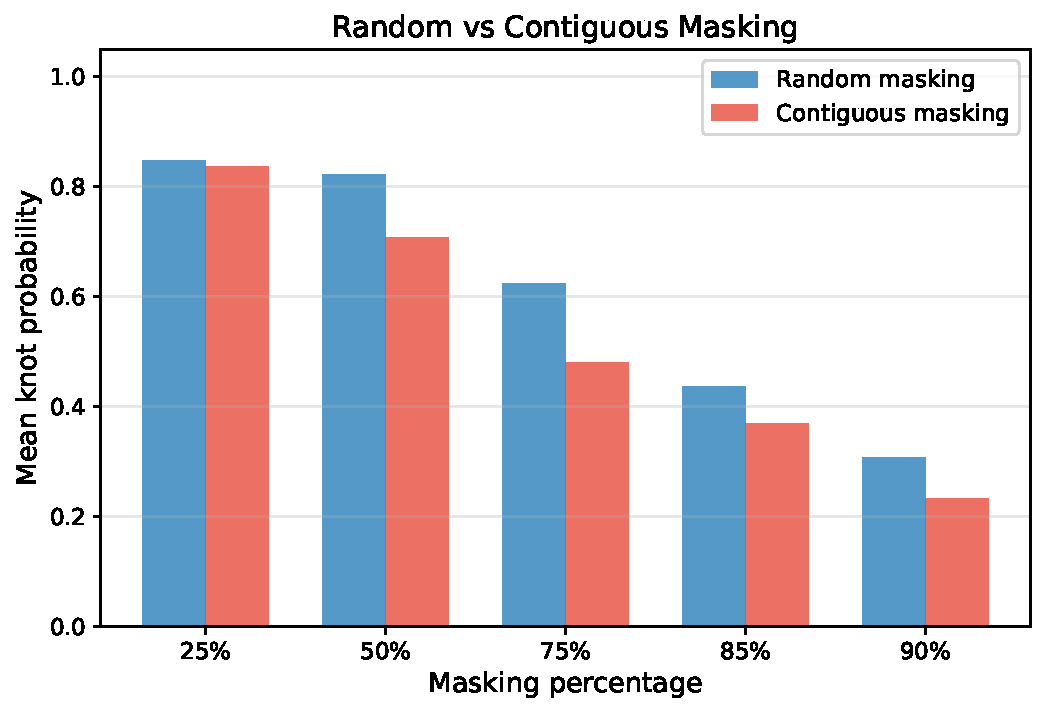
\includegraphics[width=0.85\textwidth]{figures/fig_contiguous_vs_random.pdf}
\caption{Contiguous masking versus random masking comparison.}
\label{fig:contiguous}
\end{figure}

\begin{figure}[h]
\centering
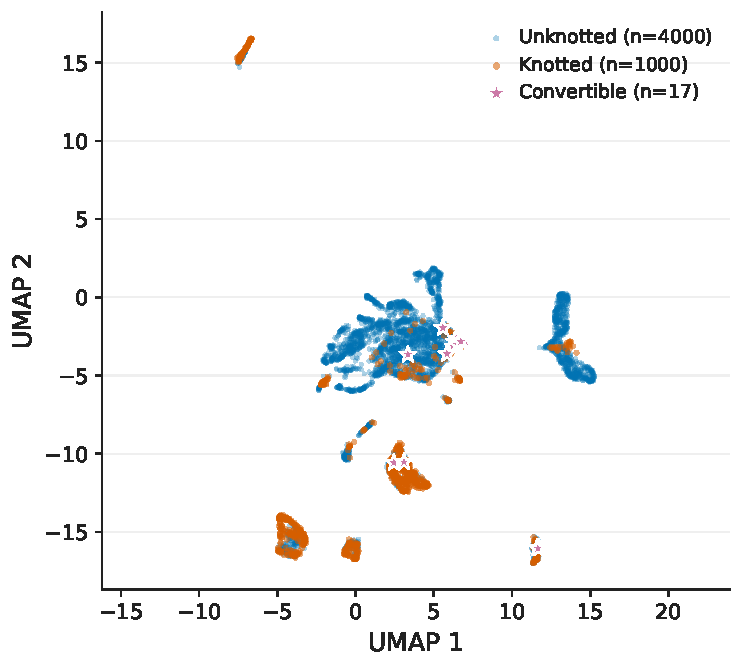
\includegraphics[width=0.85\textwidth]{figures/fig_umap_knotted.pdf}
\caption{UMAP projection of ESM3 embeddings for 5,000 real proteins. A simple MLP classifier achieves 97.1\% accuracy on this representation.}
\label{fig:umap}
\end{figure}

\begin{figure}[h]
\centering
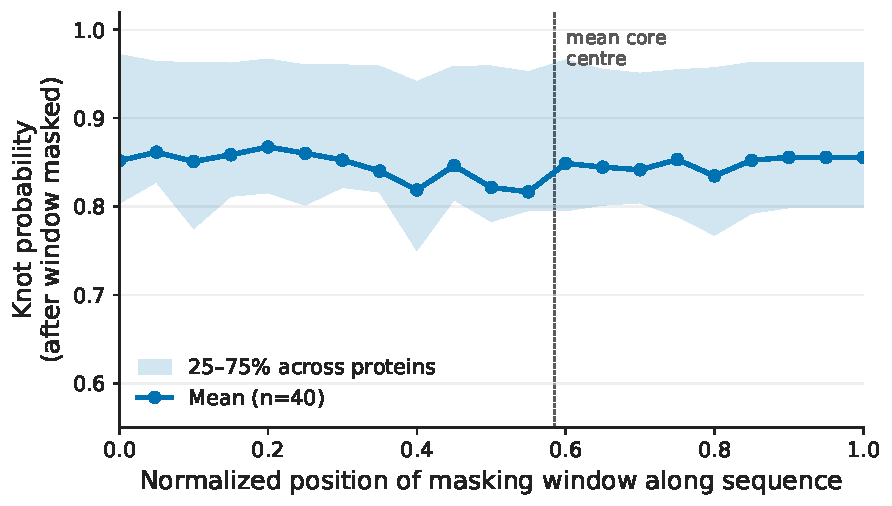
\includegraphics[width=0.9\textwidth]{figures/fig_sliding_window.pdf}
\caption{Sliding window vulnerability profile ($n=40$, window size 50 residues).}
\label{fig:sliding_window}
\end{figure}

\begin{figure}[h]
\centering
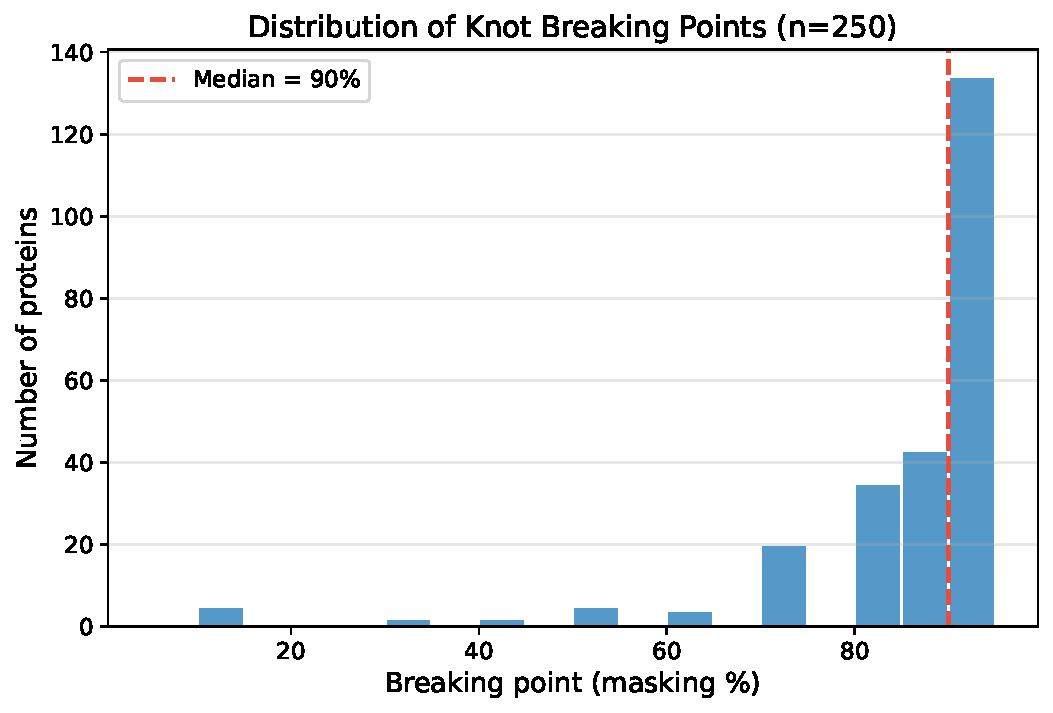
\includegraphics[width=0.85\textwidth]{figures/fig_breaking_histogram.pdf}
\caption{Distribution of breaking points across 250 knotted proteins.}
\label{fig:breaking_hist}
\end{figure}

\begin{figure}[h]
\centering
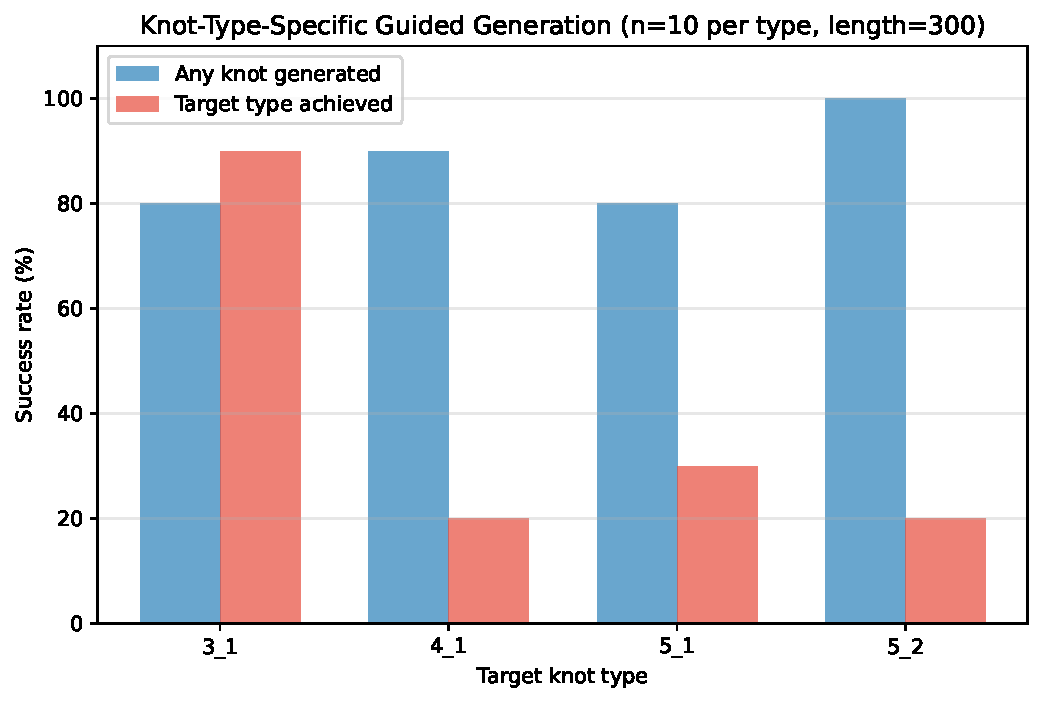
\includegraphics[width=0.85\textwidth]{figures/fig_typed_gen.pdf}
\caption{Knot-type-specific guided generation results.}
\label{fig:typed_gen}
\end{figure}

\end{document}
